\documentclass[a4paper,12pt]{report}
\usepackage[utf8]{inputenc}
\usepackage[margin=2.0cm]{geometry}
\usepackage{graphicx}

% Title Page
\title{Měření kapacity kondenzátoru}
\author{Vojtěch Vašek}
\date{\today}


\begin{document}
\maketitle
\newpage
\chapter*{Úkol měření}
\begin{itemize}
 \item [1.] {V rámci domácí přípravy nastudujte problematiku kondenzátorů jako součástek elektronických obvodů, dále problematiku elektrostatického pole a základní a charakteristické vlastnosti izolantů.}
 \item [2.] {Do závěrečných poznámek zpracujte v rámci domácí přípravy přehled druhů vyráběných kondenzátorů (výpis z katalogových listů), jejich vlastnosti, orientační cenové relace apod. Dále zpracujte přehled veličin používaných pro popis elektrostatického pole a vztahů mezi nimi.}
 \item [3.] {Změřte kapacitu kondenzátorů $C_1$, $C_2$ a $C_3$ multimetrem.}
 \item [4.] {Vypočítejte výslednou kapacitu jejich sériové a paralelní kombinace. Také hodnoty těchto kombinací změřte multimetrem.}
 \item [5.] {Změřte kapacitu jednotlivých kondenzátorů dále sériové a paralelní kombinace nepřímo Ohmovou metodou.}
 \item [6.] {Vypočítejte chybu měření kapacity.}
 \item [7.] {Zjistěte závislost proudu procházejícího kondenzátorem $C_1$ na napětí při napájení kondenzátoru střídavým napětím s konstantním kmitočtem.}
 \item [8.] {Zjistěte závislost kapacitní reaktance $X_C$ na kmitočtu $f$ v rozsahu 20 až 150 Hz.}
 \item [9.] {Výše uvedené závislosti zpracujte graficky.}
 \item [10.] {Zhodnoťte měření.}
\end{itemize}
\newpage
\chapter*{Obecná část}
Kapacity kondenzátorů lze měřit přímou metodou (nejčastěji pomocí můstku, např. Scheringova nebo multimetrem) nebo nepřímou metodou (Ohmova metoda).\\
Ohmova metoda spočívá v měření napětí na kondenzátoru a proudu jako jeho následku.
Zanedbáváme tak ztrátový činitel $tg \ \delta$.\\
V případě použití můstku je potřeba můstek kalibrovat na nulovou hodnotu podle návodu výrobce můstku.\\
V případě paralelní kombinace kondenzátorů obdržíme výslednou kapacitu součtem jednotlivých kapacit:
$$C_P = C_1+C_2+C_3+...+C_N$$
Sériová kombinace dvou kondenzátorů má celkovou kapacitu dánu vztahem:
$$C_S = \frac{C_1*C_2}{C_1+C_2}$$
Výše uvedený vztah lze jednoduše odvodit z obecného vztahu pro celkovou kapacitu sériové kombinace obecného množství kondenzátorů:
$$\frac{1}{C_S} = \frac{1}{C_1}+\frac{1}{C_2}+\frac{1}{C_3}+...+\frac{1}{C_N}$$
Kapacitní reaktance (Ohm; $\Omega$) je nepřímo úměrná kmitočtu i kapacitě kondenzátoru podle vztahu:
$$X_C = \frac{1}{\omega*C} = \frac{1}{2\pi*f*C}$$
Pro střídavě napájený ideální kondenzátor z Ohmova zákona platí:
$$X_C=Z_C=\frac{U}{I}$$
Úpravou po vzájemném dosazení výše uvedených vztahů obdržíme vztah pro kapacitu (Farad; F) měřenou nepřímo Ohmovou metodou:
$$C = \frac{I}{2\pi*f*U}$$
Měření kapacity je zatíženo chybou všech použitých měřicích přístrojů, dále chybou metody způsobenou spotřebou těchto přístrojů, chybou odečtu (zaokrouhlování) z displeje nebo stupnice. Výsledná chyba je dána součtem:
$$|\delta_C|=|\delta_{MP1}|+|\delta_{MP2}|+|\delta_{MET}|+|\delta_{G}|$$
kde $\delta_{MP1}$ je relativní chyba měřicího přístroje vypočtená za pomoci informací ze stupnice nebo manuálu měřicího přístroje, $\delta_{MET}$ je chyba metody a $\delta_G$ je relativní chyba generátoru (rozlišení vztažené k nastavenému kmitočtu).
Absolutní chybu pak lze spočítat podle vztahu:
$$\Delta_C=\frac{\delta(\%)}{100}*C_X$$
\newpage
\chapter*{Schéma zapojení}
\begin{figure}[htp]
	\begin{center}
		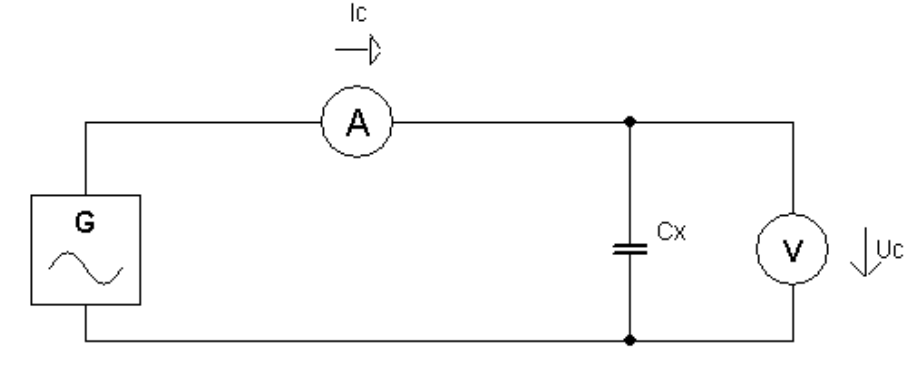
\includegraphics[scale=0.5]{ELM_27_11_23@2.png}
		\caption{Měření kapacity Ohmovou metodou}
	\end{center}
\end{figure}
\newpage
\chapter*{Postup měření}
\begin{itemize}
 \item [1.]{ Měříme kapacitu jednotlivých kondenzátorů i jejich kombinací přímo. Změřené hodnoty zapíšeme do tabulky.}
 \item [2.]{Kapacitu jednotlivých kondenzátorů i jejich kombinací měříme Ohmovou metodou; hodnoty napětí, proudu a kmitočtu zapíšeme, hodnotu kapacity, absolutní a relativní chybu měření vypočteme.}
 \item [3.]{Kondenzátor $C_1$ zapojíme do schématu, na generátoru nastavíme kmitočet 100 Hz (tuto hodnotu po celou dobu měření udržujeme), nastavujeme napětí dle tabulky, měříme a zapisujeme hodnoty proudu. Vypočteme hodnoty reaktance v závislosti na napětí. Závislost proudu na napětí zpracujeme graficky.}
 \item [4.]{Vybereme kondenzátor s největší hodnotou kapacity a zapojíme jej do schématu. Nastavíme takovou amplitudu, aby voltmetr ukazující napětí na kondenzátoru ukazoval 4~V (tuto hodnotu po celou dobu měření udržujeme, stabilitu amplitudy lze kontrolovat také pomocí osciloskopu), nastavujeme kmitočty dle tabulky, zapisujeme hodnoty proudu. Vypočteme hodnoty reaktance, závislost reaktance na kmitočtu pak zpracujeme graficky.}
\end{itemize}
\newpage
\chapter*{Otázky}
\begin{itemize}
 \item [1.]{Popište příčiny a následky tzv. "stárnutí" dielektrik.}
 \item [2.]{Popište rozdíl (z hlediska sledovaných vlastností materiálů) mezi použitím materiálu jako dielektrika a jako izolace.}
 \item [3.]{Popište vliv elektrického pole na dielektrický materiál.}
 \item [4.]{Na čem závisí linearita závislosti proudu kondenzátorem v závislosti na napětí?}
 \item [5.]{Popište základní rozdělení kondenzátorů a jejich použití.}
 \item [6.]{Popište princip změny kapacity u tzv. kapacitní diody. Kde se používá?}
 \item [7.]{Vysvětlete odchylky vypočtených a naměřených charakteristik v grafech.}
 \item [8.]{Popište konstrukci elektrolytických kondenzátorů, výhody a nevýhody jejich použití.}
 \item [9.]{Popište elektrostatické ekvivalenty Kirchhoffových zákonů známých z proudového pole.}
 \item [10.]{Definujte pojem "elektrická pevnost", popište fyzikální jevy provázející její překročení.}
 \item [11.]{Popište konstrukční provedení kondenzátorů pro vysokofrekvenční zařízení.}
\end{itemize}
\newpage
\chapter*{Tabulky naměřených hodnot}
\begin{itemize}
 \item [Tabulka 1]{Měření multimetrem (C LCR je kapacita změřená LCR můstkem, případně multimetrem, nebo jmenovitá hodnota)}
	\begin{center}
		\begin{tabular}{|c|c|}
\hline
                 & $C_{LCR}$ (F)     \\\hline
$C_1$            & 0,01 $\mu$        \\\hline
$C_2$            & 0,10 $\mu$        \\\hline
$C_3$            & 100 p             \\\hline
$C_1C_2C_3$ par. & 1.163 * $10^{-7}$ \\\hline
$C_1C_2C_3$ ser. & 9.402 n           \\\hline
		\end{tabular}
	\end{center}
 \item[Tabulka 2]{Měření Ohmovou metodou (při kmitočtu 100 Hz)}
	\begin{center}
		\begin{tabular}{|c|c|c|}
\hline
                 & $U_C$ (V) & $I_C$(A) \\\hline
$C_1$            &           &          \\\hline
$C_2$            &           &          \\\hline
$C_3$            &           &          \\\hline
$C_1C_2C_3$ par. &           &          \\\hline
$C_1C_2C_3$ ser. &           &          \\\hline
		\end{tabular}
	\end{center}
 \item[Tabulka 3]{Měření závislosti proudu na napětí}
	\begin{center}
		\begin{tabular}{|c|c|c|c|c|c|c|c|c|c|c|c|c|c|c|c|c|}
\hline
U (V)     & 0 & 0.5 & 1 & 1.5 & 2 & 2.5 & 3 & 3.5 & 4 & 4.5 & 5 & 5.5 & 6 & 6.5 & 7 & 7.5 \\\hline
$I_C$ (A) &   &     &   &     &   &     &   &     &   &     &   &     &   &     &   &     \\\hline
		\end{tabular}
	\end{center}
 \item[Tabulka 4]{Měření závislosti proudu na kmitočtu}
	\begin{center}
		\begin{tabular}{|c|c|c|c|c|c|c|c|c|c|c|c|c|c|c|}
\hline
$f$ (Hz)  & 20 & 30 & 40 & 50 & 60 & 70 & 80 & 90 & 100 & 110 & 120 & 130 & 140 & 150 \\\hline
$U_C$ (V) &    &    &    &    &    &    &    &    &     &     &     &     &     &     \\\hline
$I_C$ (A) &    &    &    &    &    &    &    &    &     &     &     &     &     &     \\\hline
		\end{tabular}
	\end{center}
\end{itemize}
\newpage
\chapter*{Výpočty a odvození}
\section*{Měření Ohmovou metodou – výpočet kapacity}
$$C_1 = \frac{I}{2\pi*f*U} = \frac{}{} = F$$
$$C_2 = \frac{I}{2\pi*f*U} = \frac{}{} = F$$
$$C_3 = \frac{I}{2\pi*f*U} = \frac{}{} = F$$
$$C_S = \frac{I}{2\pi*f*U} = \frac{}{} = F$$
	\begin{center}\textit{($C_S$ - kondenzátory $C_1C_2C_3$ spojeny sériově})\end{center}
	$$C_P = \frac{I}{2\pi*f*U} = \frac{}{} = F$$
	\begin{center}\textit{($C_P$ - kondenzátory $C_1C_2C_3$ spojeny paralelně)}\end{center}
\section*{Výpočet reaktance}
Pro kmitočet: ... Hz z tabulky 3 zachycující závislost I = I(U):
$$X_C = \frac{U}{I} = \frac{}{} = \Omega$$
Pro napětí: ... V z tabulky 4 zachycující závislost I = I(U):
$$X_C = \frac{U}{I} = \frac{}{} = \Omega$$
\newpage
\chapter*{Tabulky vypočtěných hodnot}
\begin{itemize}
 \item [Tabulka 5]{Měření Ohmovou metodou - výpočet neznámé kapacity, absolutní a relativní chyby měření kapacity}
	\begin{center}
		\begin{tabular}{|c|c|c|c|}
\hline
                 & $C_X$ (F) & $\Delta_C$ (F) & $\delta_C$ (\%) \\\hline
$C_1$            &           &                &                 \\\hline
$C_2$            &           &                &                 \\\hline
$C_3$            &           &                &                 \\\hline
$C_1C_2C_3$ par. &           &                &                 \\\hline
$C_1C_2C_3$ ser. &           &                &                 \\\hline
		\end{tabular}
	\end{center}
 \item[Tabulka 6]{Výpočet závislosti reaktance na napětí}
	\begin{center}
		\begin{tabular}{|c|c|c|c|c|c|c|c|c|c|c|c|c|c|c|c|c|}
\hline
U (V)          & 0 & 0.5 & 1 & 1.5 & 2 & 2.5 & 3 & 3.5 & 4 & 4.5 & 5 & 5.5 & 6 & 6.5 & 7 & 7.5 \\\hline
$X_C (\Omega)$ &   &     &   &     &   &     &   &     &   &     &   &     &   &     &   &     \\\hline
		\end{tabular}
	\end{center}
 \item[Tabulka 7]{Výpočet závislosti reaktance na kmitočtu}
	\begin{center}
		\begin{tabular}{|c|c|c|c|c|c|c|c|c|c|c|c|c|c|c|}
\hline
$f$ (Hz)       & 20 & 30 & 40 & 50 & 60 & 70 & 80 & 90 & 100 & 110 & 120 & 130 & 140 & 150 \\\hline
$X_C (\Omega)$ &    &    &    &    &    &    &    &    &     &     &     &     &     &     \\\hline
		\end{tabular}
	\end{center}
\end{itemize}
\newpage
\chapter*{Grafické závislosti}
\begin{figure}[htp]
	\begin{center}
		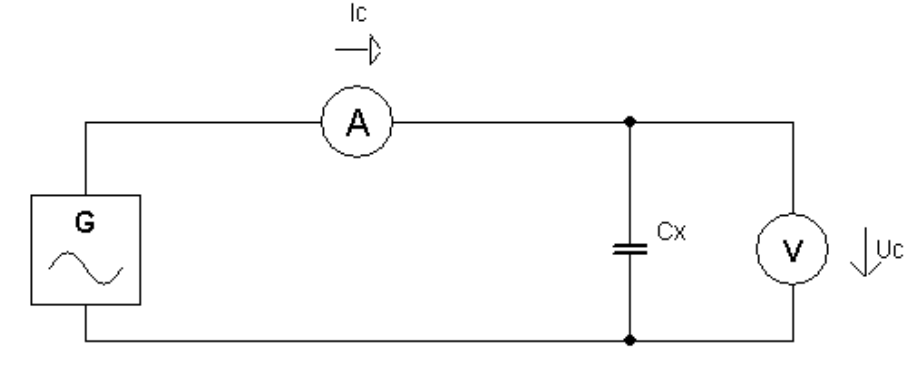
\includegraphics[scale=0.5]{ELM_27_11_23@2.png}
		\caption{ I = f(U) (index "n" značí naměřenou hodnotu, index "v" značí hodnotu vypočtenou ze jmenovité kapacity)}
		
		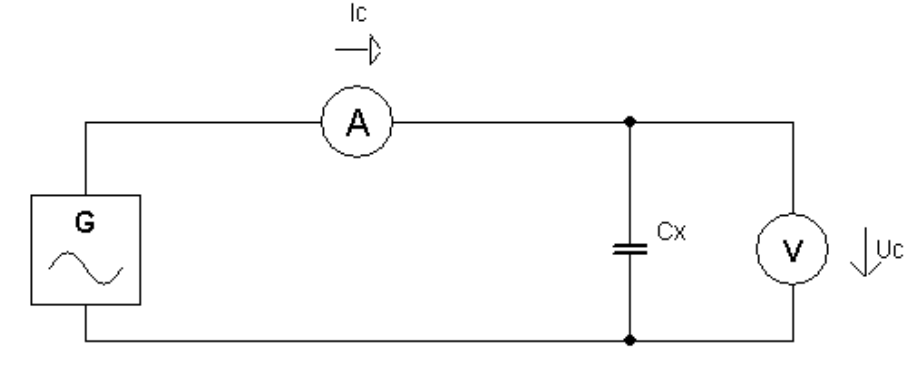
\includegraphics[scale=0.5]{ELM_27_11_23@2.png}
		\caption{ $X_C$ = f(U) (index "n" značí naměřenou hodnotu, index "v" značí hodnotu vypočtenou ze jmenovité kapacity a kmitočtu)}
		
		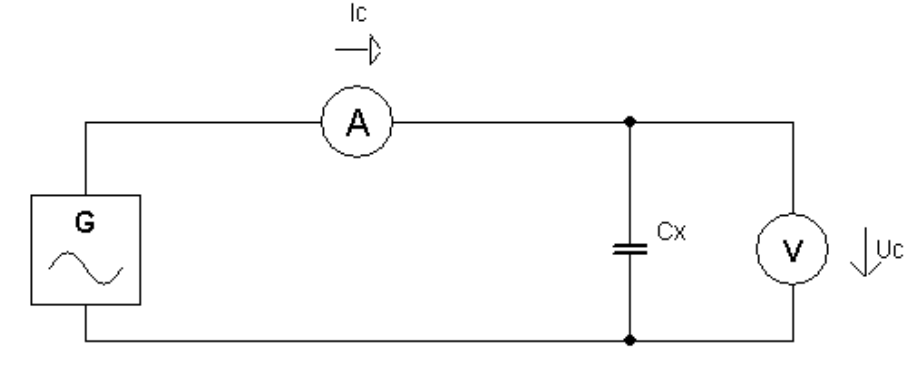
\includegraphics[scale=0.5]{ELM_27_11_23@2.png}
		\caption{ $X_C$ = f(f) (index "n" značí naměřenou hodnotu, index "v" značí hodnotu vypočtenou ze jmenovité kapacity a kmitočtu)}
	\end{center}
\end{figure}
\newpage
\chapter*{Odpovědi na otázky}
\begin{itemize}
 \item [1.]{}
 \item [2.]{}
 \item [3.]{}
 \item [4.]{}
 \item [5.]{}
 \item [6.]{}
 \item [7.]{}
 \item [8.]{}
 \item [9.]{}
 \item [10.]{}
 \item [11.]{}
\end{itemize}
\newpage
\chapter*{Závěr}
\section*{Použité informační prameny}
\begin{tabular}{|l|c|}
\hline
\textbf{Datum vypracování:} & \today \\\hline
\textbf{Čestné prohlášení:} & Prohlašuji, že jsem protokol zpracoval samostatně, veškeré použité \\
                            & prameny jsem uvedl ve stati "Použité informační prameny". \\\hline
\textbf{Podpis studenta:}   & \\
							& \\
							& \\
							& \\\hline
\end{tabular}
\section*{Použité přístroje}
	\begin{tabular}{|c|c|c|c|c|}
\hline
Přístroj     & Typ & Výrobní číslo & Inventární číslo & Poznámka \\\hline
generátor    &     &               &                  &          \\\hline
ampérmetr    &     &               &                  &          \\\hline
voltmetr     &     &               &                  &          \\\hline
kondenzátory &     &               &                  &          \\\hline
kabely       &     &               &                  &          \\\hline
multimetr    &     &               &                  &          \\\hline
	\end{tabular}
\section*{Hodnocení a přiřazení klasifikace}
\begin{tabular}{|c|c|c|c|}
\hline
\textbf{Etapa hodnocení úlohy} & \textbf{Bodovaná část}                    & \textbf{Maximální}  & \textbf{Získané} \\
                               &                                           & \textbf{počet bodů} & \textbf{body}    \\\hline
Samostatná příprava            & Ústní přezkoušení z měřené problematiky   &  10                 &                  \\\hline
Měření v laboratoři            & Zapojování schémat, průběh měření         &   5                 &                  \\\hline
Konzultace                     & Nepovinná, proběhla dne:                  &   5                 &                  \\\hline
Zpracování protokolu           & Úpravnost, struktura protokolu            &   5                 &                  \\\hline
Zpracování protokolu           & Výpočty (dosazení, výsledky, jednotky)    &   5                 &                  \\\hline
Zpracování protokolu           & Tabulky                                   &   5                 &                  \\\hline
Zpracování protokolu           & Grafy (popis os, měřítko, vlastní graf)   &  15                 &                  \\\hline
Zpracování protokolu           & Odpovědi na otázky                        &  10                 &                  \\\hline
Zpracování protokolu           & Závěr                                     &  10                 &                  \\\hline
                               & Obhajoba                                  &  30                 &                  \\\hline
\textbf{Celkové hodnocení}     & \textbf{protokolu o laboratorním cvičení} & 100                 &                  \\\hline
\end{tabular}
\\
\\
\\
\begin{tabular}{|c|c|}
 \hline
\textbf{Řádný termín}                        &                    \\
                                             &                    \\\hline
\textbf{Počet získaných bodů}                & \textbf{Hodnocení} \\\hline
0 až 49                                      & 5                  \\\hline
50 až 60                                     & 4                  \\\hline
61 až 70                                     & 3                  \\\hline
71 až 85                                     & 2                  \\\hline
86 až 100                                    & 1                  \\\hline
\textbf{Uzavření klasifikace protokolu dne:} &                    \\
                                             &                    \\
\textbf{Podpis:}                             &                    \\
                                             &                    \\
                                             &                    \\\hline

    
\end{tabular}


\end{document}          
